\chapter{Core Language Syntax and Types}
In this chapter we give the formal description of the language syntax and types. We explain what
it means for a judgement to exist as binary trees and then how we approximate the tree judgement
to a multiset inorder to simplify our type assignment algorithm.

\begin{figure}[h]
  \begin{framed}
    \begin{flalign*}
      \text{Type Variables}\ \ \      t, u, v         &\in \text{Type Variables}  \nonumber\\
      % \text{Kinds}\ \ \               \kappa          &::= \star \mid \kappa \rightarrow \kappa \nonumber\\
      % \text{Type constructors}\ \ \   T^{\kappa}       &::= \mathcal{T}^{\kappa}\ \text{where}
      %                                                 \{\overset{!}{\sepimp}, \sepimp, \xrightarrow{!}, \rightarrow \} \subseteq \mathcal{T}^{* \rightarrow * \rightarrow *}\nonumber\\
      \text{Types}\ \ \               \tau            &::= t \mid \tau \rightarrow \tau\ \text{where}\ \{\overset{!}{\sepimp}, \sepimp, \xrightarrow{!}, \rightarrow \} \subseteq \rightarrow \nonumber\\
      \text{Predicates}\ \ \          \pi             &::= \texttt{Un}\ \tau \mid \texttt{SeFun}\ \tau \mid \texttt{ShFun}\ \tau \mid \tau \geq \tau' \nonumber\\
      \text{Qualified Types}\ \ \     \rho            &::= \tau \mid \pi => \rho \nonumber\\
      \text{Type schemes}\ \ \        \sigma          &::= \rho \mid \forall t. \sigma \nonumber
    \end{flalign*}
  \end{framed}
  \caption{Types \qub{}}
  \label{fig:qub-types}
\end{figure}
% Describe types
The type language consists of type variables and four binary type constructors the
sharing arrow ($\rightarrow$) and the separating arrow ($\sepimp$) and unrestricted
version of both the arrows. The sharing arrow
would mean that the function shares resources with its argument and the separating
arrow would mean that the function does not share resources with its arguments.
We would write both the arrows in an infix notation.
% Describe Kinds
% The kind system is simple where we use $\star$ to denote all the types.
% We use $\tau$, $v$ and $\phi$ to denote types of any kind.
% We exclude additive and multiplicative product types and sum type in our core language as we can
% encode them in our core language. Extentions to \qub{} with sum types and product types is
% described in \cref{chp:datatypes}.
% The system is powerful enough to let programmers define their own {\color{red} types using the type constructors.}
% $\sepimp$ and $\rightarrow$ type constructors have a kind $\star \rightarrow \star \rightarrow \star$.
% The kind of type constructor is computed using the following rule:
% \begin{framed}
%   \begin{prooftree}
%     \AxiomC{$T :: \kappa' \rightarrow \kappa$}
%     \AxiomC{$T' :: \kappa'$}
%     \BinaryInfC{$T T' :: \kappa$}
%   \end{prooftree}
% \end{framed}
% The language of type constructors is a system of combinators without reduction rules.
% This treatement of type constructors is similar to Jones' \citeyearpar{jones_system_1993}. Inference
% mechanism for the kind of type constructors discussed in \cref{sec:kind-system}.
% Describe Predicates
The predicate system enhances the expressibility of the type system. Following the same route taken
by Quill \citep{morris_best_2016} we use the predicate \texttt{Un} $\tau$ to denote
that the type $\tau$ is unrestricted. We write \texttt{ShFun} $\tau$ to describe that type $\tau$ may share resources with its
argument types and \texttt{SeFun} $\tau$ to describe that $\tau$ is
does not share any resources from its argument types. The function types can also be of the unrestricted type.
Thus if a type $\tau$ is unrestricted i.e. it qualifies with predicate \texttt{Un} and it is also one of the function types
i.e. \texttt{SeFun} or \texttt{ShFun}, we write them as $\overset{!}{\sepimp}$ and $\xrightarrow{!}$ respectively.
This can be considered as an improving substitution following Jones notion of improvement of qualified types \citep{jones_simplifying_1995}.
We also define an ordering on types by using the predicate $\geq$. The predicate $\tau \geq \tau'$ holds if the type $\tau'$
is less restricting than $\tau$. The predicate entailment relations $P => Q$ are given in \cref{fig:entailment-rules}.

The current system does not have any kind system. They can be added into the system as a language extension
to be able to define type constructors which is described in \cref{chp:datatypes}.

\begin{figure}[h]
  \begin{framed}
    \begin{minipage}{0.20\linewidth}
      \begin{prooftree}
        \AxiomC{$\pi \in P$}
        \UnaryInfC{$P => \pi$}
      \end{prooftree}
    \end{minipage}
    \begin{minipage}{0.20\linewidth}
      \begin{prooftree}
        \AxiomC{$\bigwedge_{\pi \in Q} P => \pi$}
        \UnaryInfC{$P => Q$}
      \end{prooftree}
    \end{minipage}
    \begin{minipage}{0.20\linewidth}
      \begin{prooftree}
        \AxiomC{}
        \UnaryInfC{$P => \Un{(\tau \sepimp \tau')}$}
      \end{prooftree}
    \end{minipage}
    \begin{minipage}{0.20\linewidth}
      \begin{prooftree}
        \AxiomC{}
        \UnaryInfC{$P => \Un{(\tau \rightarrow \tau')}$}
      \end{prooftree}
    \end{minipage}
    \begin{minipage}{0.20\linewidth}
      \begin{prooftree}
        \AxiomC{$\tau = \sepimp \vee \tau = \overset{!}{\sepimp}$}
        \UnaryInfC{$P => \SeFun{\tau}$}
      \end{prooftree}
    \end{minipage}
    \begin{minipage}{0.20\linewidth}
      \begin{prooftree}
        \AxiomC{$\tau = \rightarrow \vee \tau = \overset{!}{\rightarrow}$}
        \UnaryInfC{$P => \ShFun{\tau}$}
      \end{prooftree}
    \end{minipage}
    \begin{minipage}{0.20\linewidth}
      \begin{prooftree}
        \AxiomC{$P => \Un{\tau}$}
        \UnaryInfC{$P => \tau \geq (v \overset{!}{\sepimp} v')$}
      \end{prooftree}
    \end{minipage}
    \begin{minipage}{0.20\linewidth}
      \begin{prooftree}
        \AxiomC{$P => \Un{\tau}$}
        \UnaryInfC{$P => \tau \geq (v \overset{!}{\rightarrow} v')$}
      \end{prooftree}
    \end{minipage}
    \begin{minipage}{0.5\linewidth}
      \begin{prooftree}
        \AxiomC{$$}
        \UnaryInfC{$P => \tau \geq (v \sepimp v')$}
      \end{prooftree}
    \end{minipage}
    \begin{minipage}{0.5\linewidth}
      \begin{prooftree}
        \AxiomC{$$}
        \UnaryInfC{$P => \tau \geq (v \rightarrow v')$}
      \end{prooftree}
    \end{minipage}
    \begin{minipage}{0.5\linewidth}
      \begin{prooftree}
        \AxiomC{$P => \tau \geq \phi t$}
        \AxiomC{$t\ \text{fresh}$}
        \BinaryInfC{$P => \tau \geq \phi$}
      \end{prooftree}
    \end{minipage}
    \begin{minipage}{0.5\linewidth}
      \begin{prooftree}
        \AxiomC{$P => \tau t \geq \phi$}
        \AxiomC{$t\ \text{fresh}$}
        \BinaryInfC{$P => \tau \geq \phi$}
      \end{prooftree}
    \end{minipage}
  \end{framed}
  \caption{Entailment Rules}
  \label{fig:entailment-rules}
\end{figure}


% \TODO{Need some more reading/writing about multienvironment}
% Describe Type assignments
In normal type systems, the contexts are represented as sets or lists. In \BI\ they are represented as binary trees.
The leaf nodes contain the pair of term and its associated type. Internal nodes of the context tree are
connectives which can either be a semicolon ($;$) or a comma ($,$).
If a bunch $\Delta$ is a subtree of $\Gamma$, then we denote a subtree relation by $\Gamma(\Delta)$.
Two context are equivalent ($\Gamma \equiv \Delta$)if they can be transformed into one another by renaming the identifiers.
The bunches have a restriction that no identifier appears more than once. We restrict certain structural rules on the context
depending on the connectives being used. If contexts are combined using a comma ($,$), contraction and weakening is not admissible,
but if the contexts are combined using a semicolon ($;$) then it can undergo contraction and weakening. Exchange rule is admissible
in both the connectives. This distinction enables us to have a special treatment for resources in our language.
By associating a resource with a comma constructor, our type system will not disposed it off by using the contraction rule.
While, non-resourceful objects (or normal propositions) can be combined using the semi-colon constructor.
An example bunch is shown in \cref{fig:bunches-bi}. a and b have a shared context while c is separate from the bunch a and b.
If $\Gamma$ represents the complete bunch of \cref{fig:bunches-bi}, $\Delta \equiv (a:A; b:B)$ and $\Delta' \equiv (c:C)$
then $\Gamma \equiv \Delta,\Delta'$ and $\Gamma(\Delta)$.

\begin{figure}[h]
  \centering
  \tikzset{every tree node/.style={minimum width=2em},
         blank/.style={draw=none},
         edge from parent/.style=
         {draw,edge from parent path={(\tikzparentnode) -- (\tikzchildnode)}},
         level distance=1.5cm}
\begin{tikzpicture}
\Tree
[.,
    [.;
        [.a:A ]
        [.b:B ]
    ]
    [.c:C ]
    ]
\end{tikzpicture}
\caption{Bunches in \textbf{\em BI}}
\label{fig:bunches-bi}
\end{figure}

In our system we try to generalize the tree approach into a graph where each node represents the variables or resources
and the edges between the nodes represent sharing between the variables. The example in \cref{fig:bunches-bi} can
be represented as what we would call as a sharing graph shown in \cref{fig:sharing-graph}.

\begin{figure}[h]
  \begin{framed}\centering
    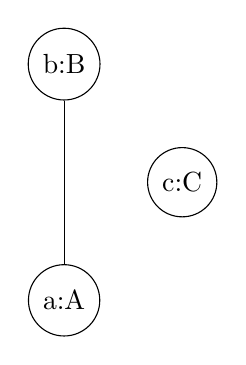
\begin{tikzpicture}
        \node[shape=circle,draw=black] (A) at (0,0) {a:A};
        \node[shape=circle,draw=black] (B) at (0,3) {b:B};
        \node[shape=circle,draw=black] (C) at (1.5,1.5) {c:C};

        \path [-] (A) edge node {} (B);
    \end{tikzpicture}
  \end{framed}
  \caption{Sharing Graph}
\label{fig:sharing-graph}
\end{figure}

We formally define $\Psi$ to be a sharing relation between variables to the collection of variables it is in sharing with.
The relation $\Psi(x, \{y_1, y_2, y_3\})$ holds if $x$ shares with $\{y_1, y_2, y_3\}$
Domain of $\Psi$ will be defined as $\texttt{dom}(\Psi) = \{x \mid (x, \bar{y}) \in \Psi \}$, where $\bar{y}$
is the collection of variables shared with $x$. One can think of $\Psi$ similar to $\Gamma$, but instead of the type of
the variable it contains the sharing information. Extending the sharing for a variable will be denoted by $\Psi(x) + y$,
which would mean the variable $y$ is in sharing with $x$. We axiomatize the sharing operation to be reflexive,
symmetric and non-transitive. So to say:
\begin{flalign*}
 &\forall_{x \in \texttt{dom}(\Psi)}\ x \in \Psi(x) \tag{reflexive}\\
 &\forall_{x,y \in \texttt{dom}(\Psi)}\ \text{if}\ y \in \Psi(x)\ \text{then}\ x \in \Psi(y) \tag{symmetric}\\
\end{flalign*}

Using the sharing graph as type assignment would make the type inferencing considerably complex.
We simplify the sharing graph into a collection of 3 tuple containg the
variable identifier, its type and a collection of variables it shares with. For example,
if a resource $x$ has type $\tau$ and it shares with variables $\{y_1, y_2, y_3\}$ we would represent it as $x^{\{y_1, y_2, y_3\}}:\tau$
or just $x^{\bar{y}}:\tau$ for short. We would write $\Gamma, x^{\bar{y}}:\tau$ to mean $\Gamma \sqcup \{x^{\bar{y}}:\tau\}$.

\begin{figure}[h]
  \begin{framed}
    \begin{flalign*}
      \text{Environments}\ \ \      \Gamma,\Delta     &::= \epsilon \mid x^{\bar{y}}:\sigma \mid \Gamma \varoplus \Delta \mid \Gamma \circledast \Delta
  \end{flalign*}
\end{framed}
  \caption{Typing Context}
  \label{fig:typing-context}
\end{figure}


\begin{figure}[h]
  \begin{framed}
    \noindent
    \begin{flalign*}
      \texttt{Vars}(\Gamma, x^{\vec{y}}) &= \texttt{Vars}(\Gamma) \cup \{ x \}\\
      \texttt{Shared}(\Gamma, x^{\vec{y}}) &= \texttt{Shared}(\Gamma) \cup \{ \vec{y} \}\\
      \texttt{Used}(\Gamma) &= \texttt{Vars}(\Gamma) \cup \texttt{Shared}(\Gamma)\\
      (\Gamma, x^{\vec{y}})^{[a \mapsto \vec{b}]} &= \begin{cases}
        x \notin \vec{y}\ \ \ \ (\Gamma^{[a \mapsto \vec{b}]}, x^{\vec{y}}:\tau)\\
        x \in \vec{y}\ \ \ \  (\Gamma^{[a \mapsto \vec{b}]}, x^{(\vec{y}\backslash a)\cup\vec{b}}:\tau)
      \end{cases}\\
      \Gamma^{[\vec{a} \mapsto \vec{b}]} &= (\dots((\Gamma^{[a_1 \mapsto \vec{b}]})^{[a_2 \mapsto \vec{b}]})^{\dots})^{[a_n \mapsto \vec{b}]}
    \end{flalign*}
  \end{framed}
  \caption{Auxilary Functions on Type Assigments}
  \label{fig:multiset-aux-function}
\end{figure}

We define a few auxilary functions on the
type assigments. \texttt{Vars}($\Gamma$) is the set of all the term variables in $\Gamma$. \texttt{Shared}($\Gamma$) computes
the set of all the term variables that are in sharing with each other. \texttt{Used}($\Gamma$) computes the
union of all the term variables in the type assignment and the term variables shared by each of those.
We define two partial operators on type assigments as shown in \cref{fig:type-assignment-operations}.
The mapping function ($\Gamma^{[\vec{a} \mapsto \vec{b}]}$) extends the sharing relation between the terms. In the sharing graph perspective
it would mean adding edges between the nodes. Two type assigments are said to be in disjoint union ($\circledast$)
if either of the type assignments used terms are not in common
with other type assignment's shared term. If the type assignments have an exact overlapping of terms being used,
it is said to be in a sharing union ($\varoplus$). The ($\#$) in ($\circledast$) represents disjoint check and we use
the standard notion of set equality for checking sharing union.


\begin{figure}[h]
  \begin{framed}
    \begin{flalign*}
      \Gamma \circledast \Gamma' &= \Gamma \sqcup \Gamma' =>
           \texttt{if}\ \texttt{Vars}(\Gamma) \# \texttt{Used}(\Gamma') \wedge \texttt{Vars}(\Gamma')\# \texttt{Used}(\Gamma) \\
      \Gamma \varoplus \Gamma'   &= \Gamma \sqcup \Gamma' => \texttt{if}\ \texttt{Used}(\Gamma) = \texttt{Used}(\Gamma')
    \end{flalign*}
  \end{framed}
  \caption{Type Assignment Operations}
  \label{fig:type-assignment-operations}
\end{figure}


\begin{figure}[h]
  \begin{framed}
    \begin{flalign*}
      \text{Term Variables}\ \ \  x, y, z  &\in \text{Var} \nonumber\\
      % \text{Patterns}\ \ \        p        &::= x \mid C \vec{x}\nonumber\\
      \text{Expressions}\ \ \     M, N     &::= x \mid \lambda^{*}x. M \mid \lambda^{\alpha}x. M \mid M N \mid \Let{x}{M}{N}\nonumber
      %&\mid \Case{M}{\{\texttt{inl}\ x \mapsto N ; \texttt{inr}\ y \mapsto N'\}}\mid \texttt{inl}\ x \mid \texttt{inr}\ y \nonumber\\
     % &\mid  \mid \Pair{M,N} \mid \Pair{M;N}
    \end{flalign*}
  \end{framed}
  \caption{Language Syntax}
  \label{fig:quill-terms}
\end{figure}
% Describe the language here

% Describe terms and patterns
Our term language is similar to that of simply typed lambda calculus involving variables and application
but we have two types of lambda expressions, the alpha lambda ($\lambda^{\alpha}$) denotes sharing
of the argument term with the expression $M$ and the separating lambda term ($\lambda^{*}$) that implies
the argument term has a separating context with the expression $M$. We also have polymorphic $\texttt{let}$
expressions to be able to define expressions with a limited scope.  % The type constructors \texttt{inl} and \texttt{inr} build
% a sum type while \texttt{case} expression match on the sum type to specify what should be done in for the two ways
% in which the sum type was created.

% The type constructors are added in order to allow programmers to define their own data types. They can be used to define sum and product types.
% \texttt{case} expression can be used to pattern match on the expression to express it in terms
% of individual sum types. Patterns are either term variables or constructor terms.

%%% Local Variables:
%%% mode: latex
%%% TeX-master: "../thesis-ku.tex"
%%% End:
 